\documentclass{article}
\usepackage[utf8]{inputenc}
\usepackage{setspace}
\usepackage{gensymb}
\singlespacing
\usepackage[cmex10]{amsmath}
\usepackage{caption}

\usepackage{amsthm}

\usepackage{mathrsfs}
\usepackage{txfonts}
\usepackage{stfloats}
\usepackage{bm}
\usepackage{cite}
\usepackage{cases}
\usepackage{subfig}

\usepackage{longtable}
\usepackage{multirow}
\usepackage{fancyhdr}
\usepackage{enumitem}
\usepackage{mathtools}
\usepackage{steinmetz}
\usepackage{tikz}
\usepackage{circuitikz}
\usepackage{verbatim}
\usepackage{tfrupee}
\usepackage[breaklinks=true]{hyperref}
\usepackage{graphicx}
\usepackage{tkz-euclide}

\title{Assignment 3 - Problem 56 Dec-2018 Paper}
\author{Vishnu Gollamudi - AI22MTECH02001}
\pagestyle{fancy}
\fancyhf{}
\rfoot{https://github.com/vishnu-g1997/AI5030-course }

\begin{document}
\section{Question}
49. A standard fair die is rolled until some face other than 5 or 6 turns up. Let X denote the face value of the last roll, and A = [X is even] and B = [X is at most 2]. Then.\\
1. $P(A \bigcap B) = 0$ \\
2. $P(A \bigcap B) = 1/6$ \\
3. $P(A \bigcap B) = 1/4$ \\ 
4. $P(A \bigcap B) = 1/3$ \\

Answer: 3

\section{Solution}

\subsection{Axioms and Formulae}

\begin{enumerate}
    \item $P(X=x,Y=y)$ = $P(X=x/Y=y) \times P(Y=y)$
    \item $P(X=x)$ = $\sum_{Y_j\in R} P(X=x) P(Y=y_j)$  
\end{enumerate}

\subsection{Given Info}
\begin{enumerate}
    \item Given X is the face value of the dice\\
\item 
\begin{align*}
&  P[(X \in (2,4,6), X \in (1,2))/T] \\
&= P[(X = 2)/T] \\
&= \frac{1}{6} 
\end{align*}
\end{enumerate}

\subsection{Joint Probability}
Joint Probability of $X=2$ and T (i.e Trail is allowed )
\begin{align*}
P(X=2,T_1) &= P(X=2/T_1)  P(T_1) = \frac{1}{6} \times 1 \\
P(X=2,T_2) &= P(X=2/T_2)  P(T_2) \\
           &=\frac{1}{6} \times P(X_1 \in \{5,6\} ) = \frac{1}{6} \times \frac{1}{3}\\
P(X=2,T_i) &= P(X=2/T_i) P(T_i) = \frac{1}{6} \times \frac{1}{3^{i-1}}
\end{align*}
Probability that trail is continued till $i^{th}$ time 
\begin{equation*}
    P(T_i) = \Pi_{i=1}^{i-1} P(X_i \in \{5,6\})= \frac{1}{3^{i-1}}
\end{equation*}


\subsection{Joint Probability}
Marginal probability of P(X=2)
\begin{align*}
    P(X=2) &= \sum_{i=1}^\infty P(X=2,T_i) = \sum_{i=1}^\infty  P(X=2/T_i) \times P(T_i) \\
       &= \frac{1}{6} \times (1+\frac{1}{3}+\frac{1}{3^2} + ....+\frac{1}{3^{i-1}} + .... + \infty)\\
        &= \frac{1}{6} \times \frac{1}{1-\frac{1}{3}}\\
        &= \frac{1}{6} \times \frac{3}{2} \\
        &= \frac{1}{4}
\end{align*}

\subsection{Markov Chain Monte Carlo}
\large Markov chain model for infinite number of trails\\
\\
\vspace{20pt}
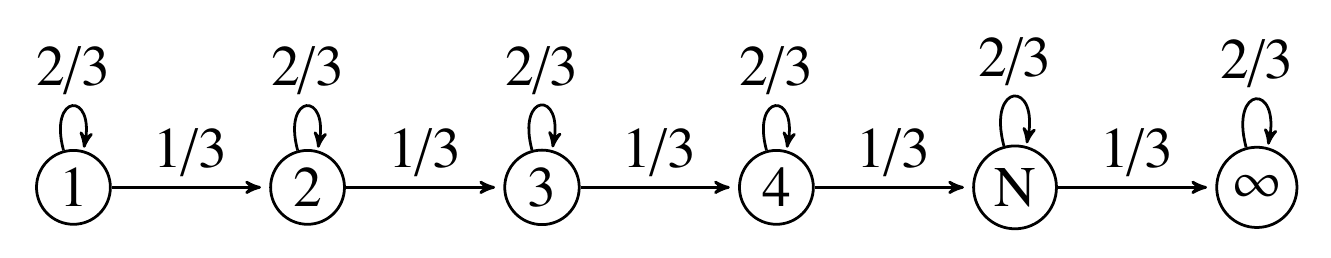
\begin{tikzpicture}[->,>=stealth',shorten >=3pt, line width=1pt, 
                                  node distance=2cm, style ={minimum size=5mm}]
\tikzstyle{every node}=[font=\huge]
\node [circle, draw] (a) {1};
\node [circle, draw] (b) [right=of a] {2};
\node [circle, draw] (c) [right=of b] {3};
\node [circle, draw] (d) [right=of c] {4};
\node [circle, draw] (e) [right=of d] {N};
\node [circle, draw] (f) [right=of e] {$\infty$};

\path  (a) edge [loop above] node {2/3} (a);
\path  (b) edge [loop above] node {2/3} (b);
\path  (c) edge [loop above] node {2/3} (c);
\path  (d) edge [loop above] node {2/3} (d);
\path  (e) edge [loop above] node {2/3} (e);
\path  (f) edge [loop above] node {2/3} (f);

\path[->] (a) edge node[above] {1/3} (b);
\path[->] (b) edge node[above] {1/3} (c);
\path[->] (c) edge node[above] {1/3} (d);
\path[->] (d) edge node[above] {1/3} (e);
\path[->] (e) edge node[above] {1/3} (f);
\end{tikzpicture}

\begin{enumerate}
    \item Since infinite number of trails are allowed, the Markov chain has infinite states
    \item Also state transition matrix will have infinite dimensions
\end{enumerate}

\textbf{State Transition matrix}\\
\begin{align*}
\begin{bmatrix}
   &2/3  &1/3& &0&    &0&  &0& ......\\
   &0   &2/3& &1/3&  &0&  &0& ...... \\
   &0   &0&   &2/3& &1/3&  &0& ......\\
   &0   &0&   &0&   &2/3& &1/3&  ..... \\
     &.   &.    &.    &.    &.  &. ......\\
     &.   &.    &.    &.    &.  &. ......\\
     &.   &.    &.    &.    &.  &. ......\\
\end{bmatrix}
\end{align*}
\end{document}
